\documentclass[14pt,a4paper]{extarticle}%
\usepackage{amsthm}
\usepackage{amsmath}
\usepackage{amsfonts}
\usepackage{amssymb}
\usepackage{setspace}
\usepackage{listings}
\usepackage{graphicx}
\usepackage{indentfirst}
\usepackage{booktabs}
\usepackage{float}
\usepackage{longtable}
\usepackage[normalem]{ulem}
\usepackage[T2A]{fontenc}
\usepackage[utf8]{inputenc}
\usepackage[english,russian]{babel}
%-------------------------------------------
\setlength{\textwidth}{7.0in}
\setlength{\oddsidemargin}{-0.35in}
\setlength{\topmargin}{-0.5in}
\setlength{\textheight}{9.0in}
\setlength{\parindent}{0.3in}
\graphicspath{{../plot/}}


\newtheorem{theorem}{Theorem}
\newtheorem{task}[theorem]{Задача}
\addto\captionsrussian{\renewcommand*{\proofname}{Решение}}

\onehalfspacing


\begin{document}

\begin{titlepage}
  \begin{center}
    МИНОБРНАУКИ РОССИИ\\
    САНКТ-ПЕТЕРБУРГСКИЙ ГОСУДАРСТВЕННЫЙ\\
    ЭЛЕКТРОТЕХНИЧЕСКИЙ УНИВЕРСИТЕТ\\
    <<ЛЭТИ>> ИМ. В. И. ЛЕНИНА (УЛЬЯНОВА)\\
    Кафедра МО ЭВМ

    \vspace{4cm}

    ОТЧЕТ\\
    по практической работе №5\\
    по дисциплине <<Теория принятия решений>>\\
    Тема: Преобразование координат
    \vfill

    \begin{tabular}{ c c c }
      Студент гр. 8303 & \uline{\hspace{3cm}} & Гришин К. И. \\[1cm]
      Преподаватель    & \uline{\hspace{3cm}} & Попова Е. В. \\
    \end{tabular}
    
    \vfill
    Санкт-Петербург\\
    2022
  \end{center}
\end{titlepage}


\section{Цель работы}
Используя программный модуль \textit{Coco}, исследовать задачу
преобразования острономических координат.

\section{Выполнение работы}

\subsection{Циклическое преобразование координат}
Вводные данные (рис. \ref{fig:input}):

\begin{figure}[H]
  \centering
  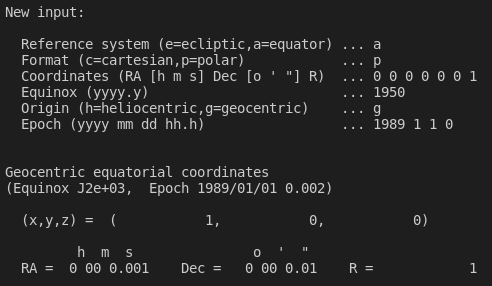
\includegraphics[scale=1.0]{input.png}
  \caption{Введеные в Coco данные}
  \label{fig:input}
\end{figure}

\begin{enumerate}
  \item Reference System - Equator
  \item Format - Polar
  \item Coordinates - 0 0 0 0 0 0 1
  \item Equinox - 1950
  \item Origin - Geocentric
  \item Epoch - 1989 1 1 0 0
\end{enumerate}

Проведено преобразование точки весенного равноденствия к новой эпохе 2000
(рис. \ref{fig:new_equinox})

\begin{figure}[H]
  \centering
  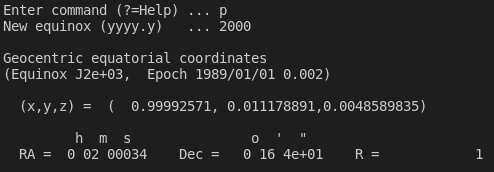
\includegraphics[scale=1.0]{new_equinox.png}
  \caption{Преобразование точки весеннего равноденствия}
  \label{fig:new_equinox}
\end{figure}

Проведено преобразование в эклиптические координаты (рис. \ref{fig:ecl})

\begin{figure}[H]
  \centering
  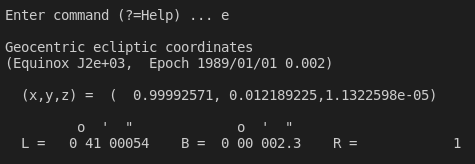
\includegraphics[scale=1.0]{ecliptic.png}
  \caption{Преоразование в эклиптические координаты}
  \label{fig:ecl}
\end{figure}

\clearpage

Проведено преобразование в гелиоцентрические координаты (рис. \ref{fig:helio})

\begin{figure}[H]
  \centering
  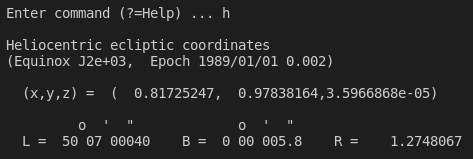
\includegraphics[scale=1.0]{helio.png}
  \caption{Преобразование в гелиоцентрические координаты}
  \label{fig:helio}
\end{figure}

Проведено обратноне преобразование в экваториальные координаты (рис. \ref{fig:equ})

\begin{figure}[H]
  \centering
  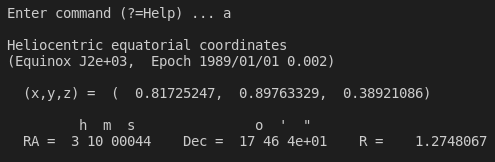
\includegraphics[scale=1.0]{equatorial.png}
  \caption{Преобразование в экваториальные координаты}
  \label{fig:equ}
\end{figure}

\clearpage

Проведено обратноне преобразование точки весеннего равноденствия к эпохе 1950
(рис. \ref{fig:old_equinox})

\begin{figure}[H]
  \centering
  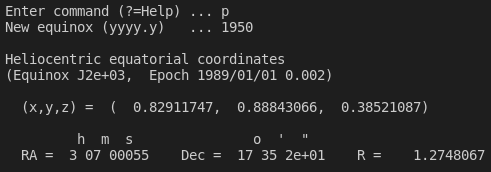
\includegraphics[scale=1.0]{old_equinox.png}
  \caption{Преобразование точки весеннего равноденствия к 1950}
  \label{fig:old_equinox}
\end{figure}

Проведено обратное преобразование к геоцентрическим координатам (рис. \ref{fig:geo})

\begin{figure}[H]
  \centering
  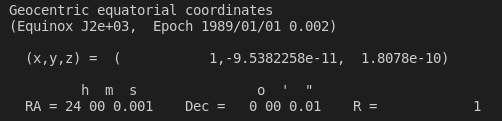
\includegraphics[scale=1.0]{geo.png}
  \caption{Преобразование в геоцентрические координаты}
  \label{fig:geo}
\end{figure}


После циклического преобразования, координаты слегка изменились.
Это объясняется тем, что числа с плавающей точкой внутри ЭВМ недостаточно точны,
а использование иррациональных чисел вовсе невозможно.

Было проведено 30 испытаний (табл. \ref{tbl:tries}) над изменением радиус-вектора координат до преобразования
и после. В каждом испытании значение RA увеличвалось на полчаса, начиная с 0ч 00мин.
График зависимости погрешности от номера испытания показан на рисунке \ref{fig:error}.

\begin{table}[H]
  \centering
  \begin{tabular}{cccccccc}
    \toprule
    {} & H &  m &      s &      $\deg$ &   ' &    '' & R \\
    \midrule
    1  &   0 &   0 &  0 &  0 &  0 &  0 & 1 \\
    2  &   0 &   30 &  0 &  0 &  0 &  0 & 1 \\
    3  &   1 &   0 &  0 &  0 &  0 &  0 & 1 \\
    4  &   1 &   30 &  0 &  0 &  0 &  0 & 1 \\
    5  &   2 &   0 &  0 &  0 &  0 &  0 & 1 \\
    ...  &   ... &   ... &  ... &  ... &  ... &  ... & ... \\
    26  &   12 &   30 &  0 &  0 &  0 &  0 & 1 \\
    27  &   13 &   0 &  0 &  0 &  0 &  0 & 1 \\
    28  &   13 &   30 &  0 &  0 &  0 &  0 & 1 \\
    29  &   14 &   0 &  0 &  0 &  0 &  0 & 1 \\
    30  &   14 &   30 &  0 &  0 &  0 &  0 & 1 \\
    \bottomrule
  \end{tabular}
  \caption{Испытания}
  \label{tbl:tries}
\end{table}

\begin{figure}[H]
  \centering
  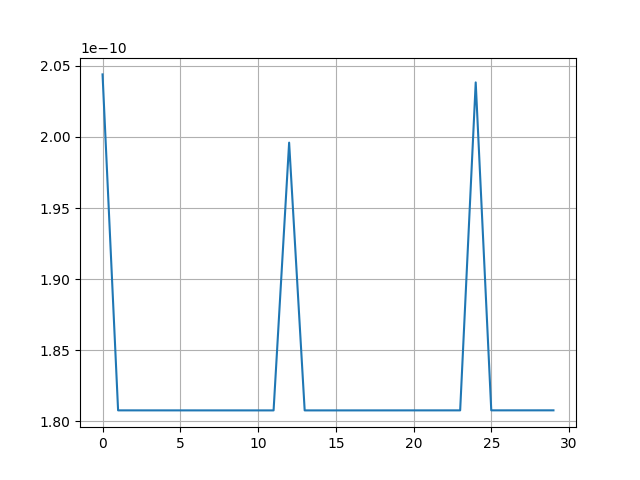
\includegraphics[scale=0.8]{Figure_1.png}
  \caption{Зависимость погрешности от значения RA}
  \label{fig:error}
\end{figure}

Из графика видно, что погрешность колеблется от $1.808\cdot10^{-10}$ до $2.044\cdot10^{-10}$.
Причем большую часть наблюдений погрешность равна $1.808\cdot10^{-10}$, а корреляция между
размером погрешности и значением RA отсутствует.

Исходный код процедуры представлен в приложении А.
Процедура используется следующим образом
\begin{lstlisting}[basicstyle=\small,language=c++]
  //
  // Variables
  //
  Position  Pos;
  char      c;
  bool      End = false;
  double    Year;

  
  // Header
  cout << endl
       << "                COCO: coordinate conversions       " << endl
       << "        (c) 1999 Oliver Montenbruck, Thomas Pfleger" << endl
       << endl;

  
  // Initialization   
  Pos.Input();
  Pos.Print();

  // Repeating procedure
  repeatance(Pos);
\end{lstlisting}

\clearpage

\subsection{Решение задачи}
Задано календарное время $X$. Вывести значение юлианской и модифицированной юлианской даты.

$X$ взят равным 1986y 04m 26d 1h 23m 0s.

Юлианская дата: $2.44655e+06$

Модифицированная юлианская дата: $46546.1$

Исходный код приведен в приложении Б.


\section{Вывод}
Были изучены различные системы координат,
применяемые для решения астрономических задач,
а также исследована возникающая погрешность
при пересчетах из одной системы координат в другую.


\clearpage

\begin{center}
  \textbf{ПРИЛОЖЕНИЕ А}
\end{center}

\begin{lstlisting}[language=c++]
  void repeatance(const Position& pos) {
    Position init_pos = pos;
    
    for (int i = 0; i < 30; i++) {
      double RA = 15.0 * Rad * Ddd(i/2, i%2*30, 0);
      double dec = Rad * Ddd(0, 0, 0);
      init_pos.m_R = Vec3D(Polar(RA, dec, 1.0));

      Position p = init_pos;
      std::cout << "======== " << i << " begin ========"
                <<std::endl;
      p.Print();
      p.SetEquinox(0);
      p.SetRefSys(Ecliptic);
      p.SetOrigin(Heliocentric);
      p.SetRefSys(Equator);
      p.SetEquinox((1950.0 - 2000.0)/100.0);
      p.SetOrigin(Geocentric);
      p.Print();
      std::cout << "======== " << i << " end ==========\n"
                << std::endl;
    }
  }
\end{lstlisting}


\clearpage

\begin{center}
  \textbf{ПРИЛОЖЕНИЕ Б}
\end{center}

\begin{lstlisting}[language=c++]
  std::cout << "date: 1986y 04m 26d 1h 23m 0s" << std::endl;
  double mjd = Mjd(1986, 4, 26, 1, 23, 0);
  double jd = mjd + 2400000.5;

  std::cout << "jd:  " << jd << std::endl;
  std::cout << "mjd: " << mjd << std::endl;
\end{lstlisting}

\end{document}